\documentclass[a4paper,12pt, oneside]{book}
\usepackage[italian]{babel}
\usepackage[utf8]{inputenc}
\usepackage[top=1in, left=1.25in, right=1.25in, bottom=1in]{geometry}

%Includes "References" in the table of contents
\usepackage[nottoc]{tocbibind}

\usepackage{url}

\usepackage{graphicx}
\usepackage{fancyhdr}
\fancypagestyle{}{
\fancyfoot[C]{\thepage}}
\pagestyle{plain}
\renewcommand{\headrulewidth}{0pt}

\usepackage{pdfpages}

%Title, date an author of the document
\title{Smart card e token crittografici}
\author{Valerio Volpe}

%Begining of the document
\begin{document}
\mainmatter

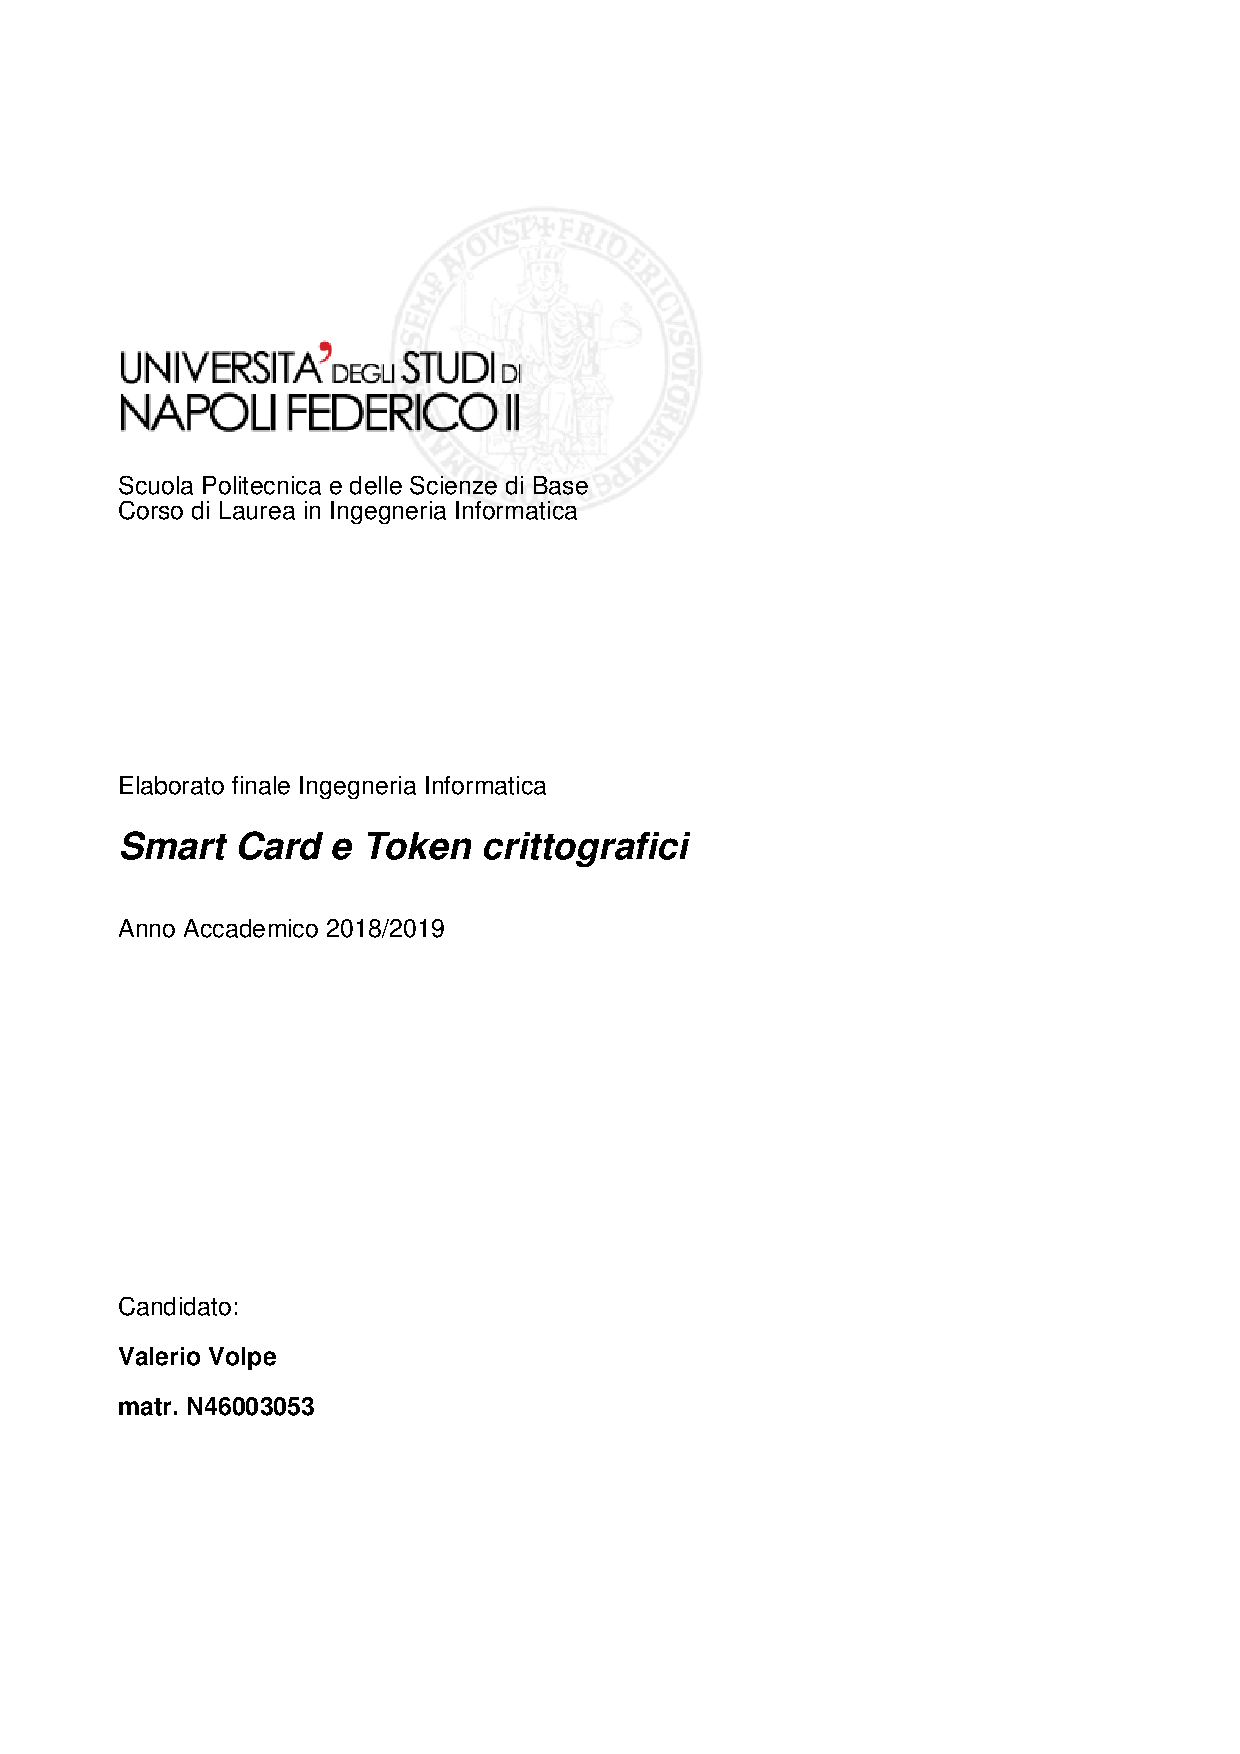
\includepdf[page={1}]{frontespizio}

\chapter*{}

\begin{flushright}%
  \emph{A tutti coloro che mi hanno sostenuto in questo percorso, in particolare alle mie nonne che non vedono l'ora di vedermi laureato}
  \thispagestyle{empty}
\end{flushright}



\tableofcontents
%\listoftables
%\listoffigures

\medskip

\chapter*{Introduzione}
\label{introduction}
\addcontentsline{toc}{chapter}{Introduzione}
Quello della sicurezza informatica è un settore molto importante e in continua evoluzione.

La crittografia gioca un ruolo fondamentale in questo campo in quanto la trasmissione dei dati viene spesso effettuata tramite canali poco sicuri e facilmente intercettabili.

I pilastri sui quali si basa la sicurezza, ovvero le problematiche che si cerca di risolvere tramite la crittografia, sono quattro:

\begin{itemize}
    \item \textbf{Riservatezza} di un messaggio, ovvero la garanzia che un messaggio possa essere letto solo dal destinatario, evitando che possa essere intercettato e letto da entità non desiderate.
    \item \textbf{Integrità} del contenuto. Il messaggio inviato deve arrivare al destinatario senza subire modifiche o manipolazione da parte di terzi.
    \item \textbf{Autenticazione} della persona con la quale si sta comunicando. Si vuole garantire che un'entità sia effettivamente ciò che dice di essere.
    \item \textbf{Disponibilità dei servizi}. Questa problematica riguarda in particolare le aziende che hanno server accessibili pubblicamente e che quindi possono essere soggetti di attacchi DoS (\textit{Denial of Service})
\end{itemize}

Per far fronte a queste problematiche (in particolare le prime tre) sono stati sviluppati vari algoritmi di crittografia, come ad esempio algoritmi a chiave simmetrica o a doppia chiave (pubblica e privata).

Come verrà illustrato nel capitolo \ref{chapter1} di questa tesi le smart card rivestono un ruolo fondamentale nel campo della crittografia e sono utilizzate in molti ambiti, come quello della telefonia mobile (paragrafo \ref{applet_sim}), del settore bancario (paragrafo \ref{carta_di_credito}) o nella più recente carta d'identità elettronica (discussa nel paragrafo \ref{carta_identita_elettronica}).

Nel capitolo \ref{chapter2} verrà illustrato più nel dettaglio il funzionamento di una smart card parlando dello standard ISO 7816 al quale risponde nel paragrafo \ref{standard} e accennando alla programmazione delle Java Card nel paragrafo \ref{java_card} e allo Smart Card Web server (paragrafo \ref{smart_card_web_server}).

Il capitolo \ref{chapter3} illustra altre tecnologie utilizzate nel settore della crittografica, in particolare si accennerà al \textit{Trusted Platrofm Module} nel paragrafo \ref{trusted_platform_module}.


\chapter{Introduzione}
\label{chapter1}

\section{Cosa sono le smart card}
Una smart card è un dispositivo hardware realizzato su un supporto di plastica in grado di elaborare e memorizzare dati, rispondendo anche ad elevati standard di sicurezza.

La prima idea di realizzare questo tipo di dispositivi è venuta nel 1968 a due inventori tedeschi: Jürgen Dethloff e Helmut Grötrupp. Da allora, grazie alle nuove tecnologie che hanno permesso di realizzare dispositivi sempre più piccoli e potenti, tale tecnologia si è diffusa proprio grazie alla sua versatilità.

Gli utilizzi delle smart card sono molteplici, dal settore bancario, a quello della telefonia, dell'identità, fino ad arrivare nel mondo del trasporto, con l'utilizzo di biglietti elettronici.
\cite{wiki_sc}

\section{Caratteristiche  delle smart card}

Ci sono due criteri che permettono di classificare le smart card. Basandoci sulle potenzialità del circuito possiamo definire le smartcard a sola memoria o a microprocessore. Invece il tipo di interfaccia di collegamento ci permettono di distinguere smartcard a contatto, senza contatto e con antenna e contattiera (ovvero a doppia interfaccia).

Le smart card a sola memoria hanno la capacità di memorizzare informazioni che possono essere lette successivamente, mentre le card a microprocessore possono effettuare elaborazioni. Infine le smarcard a contatto hanno dei pin connettori tramite i quali possono essere alimentate ed è possibile inviare e ricevere informazioni. Mentre quelle senza contatto hanno a disposizione un'antenna che reagisce a un particolare campo elettromagnetico emesso da un dispositivo di lettura/scrittura.

Le smart card rispondono allo standard ISO 7816 che definisce le caratteristiche che devono avere le card a contatto, mentre altri standard sono usati per le card senza contatto (ISO 14443 e ISO 15693).

Le smart card a microprocessore sono particolarmente utilizzate per conservare in maniera sicura una chiave privata. Grazie alla loro capacità di elaborazione sono in grado di ricevere una piccola quantità di dati (come ad esempio un hash di un documento) e restituirlo crittografato con la chiave privata contenuta al loro intero. In questo modo la chiave non "esce" mai dal microprocessore, e quindi non può essere letta in alcun modo. Grazie a questa caratteristica le smart card costituiscono un elemento sicuro per la firma digitale di documenti.
\cite{wiki_sc}

\section{Le smart card nella firma digitale}
Come accennato nel paragrafo precedente, uno degli utilizzi delle smartcard più frequente è quello nell'ambito della firma digitale.

La firma digitale è un insieme di metodi crittografici che servono a garantire l'autenticità di un messaggio trasmesso su canali non sicuri. Offrendo al destinatario tre garanzie:
\begin{itemize}
    \item L'autenticazione del mittente.
    \item La non negazione di invio del messaggio da parte dell'utente.
    \item L'integrità del messaggio inviato.
\end{itemize}

La firma digitale si basa su un sistema di cifratura asimmetrica (ovvero che utilizza due chiavi, una pubblica e una privata). La chiave privata è utilizzata per "firmare" il file, mentre quella pubblica, disponibile a chiunque, per la verifica della validità della firma.

Il classico funzionamento di una firma digitale consiste in pochi semplici step.
\begin{enumerate}
    \item Tramite una funzione di hash viene generata una stringa identificativa univoca al file. File uguali generano la stessa stringa (se viene usata la stessa funzione di hash) ed ogni stringa identifica univocamente un file.
    \item La stringa generata con la funzione di hash viene crittografata usando la chiave privata. Una volta cifrata, la firma viene allegata al documento, che risulta firmato.
    \item Per verificare l'autenticità della firma e l'integrità del documento il ricevente può calcolare nuovamente la funzione di hash del file e decifrare la firma allegata usando la chiave pubblica del mittente. Se il documento non è stato alterato e la chiave pubblica usata per decifrare la firma corrisponde alla chiave privata usata dal mittente, allora la stringa di hash calcolata corrisponderà alla stringa decifrata. Ciò garantisce i tre parametri riportati sopra.
\end{enumerate}

La chiave pubblica è solitamente fornita da una Certification Autority (CA) che garantisce che si tratti effettivamente della chiave pubblica del mittente del messaggio.

Il ruolo che la smart card gioca nella firma digitale consiste nel conservare la chiave privata in un luogo sicuro. Il codice è infatti salvato sulla memoria del chip presente sulla card, che poi viene reso inaccessibile dall'esterno. Una volta collegata la card a un calcolatore, tramite un apposito lettore, al momento della firma viene inviato alla card la stringa identificativa del file. La scheda provvederà poi a crittografare la stringa e a restituire il risultato dell'elaborazione al PC che provvederà infine ad allegare la vera e propria firma al documento.
\cite{Wiki_fd}

\section{La smart card nella telefonia mobile}
Un altro utilizzo molto frequente delle smart card è quello nell'ambito della telefonia mobile.

Viene detta SIM (dall'inglese Subscriber Identity Module) una smart card che viene inserita in un telefono cellulare e utilizzata dagli operatori telefonici per conservare in modo sicuro il codice identificativo dei loro clienti (l'IMSI che corrisponde alla sigla inglese International Mobile Subscriber Identity).

Le caratteristiche tipiche di una smart card SIM sono riassunte nella tabella \ref{parametri_SIM}.

\begin{table}
\centering
\begin{tabular}{ |c|c| } 
 \hline
 Descrizione &  64K JavaCard 2.1.1 WIB1.3 USIM \\
 \hline
 Piattaforma & Atmel AT90SC25672RU \\ 
 \hline
 Architettura CPU & 8-bit AVR \\ 
 \hline
 Tecnologia & 0.15uM CMOS \\ 
 \hline
 ROM & 256KB \\
 \hline
 Memoria non volatile & 72 KB EEPROM \\
 \hline
 RAM & 6Kb \\
 \hline
 Frequenza operativa interna & 20-30 MHz \\
 \hline
 Tempo di vita & 500mila cicli di letture/scrittura \\
 \hline
 
\end{tabular}
\caption{Tabella dei parametri tipici di una smart card SIM \cite{secret_life}.}
\label{parametri_SIM}
\end{table}

L'utilizzo che viene fatto delle sim dagli operatori è quello di fornire vari servizi ai loro clienti e controllarne l'utilizzo.

La carta SIM non contiene in memoria il numero telefonico associato all'utente, ma solo il codice identificativo IMSI ed è compito dell'operatore associarlo ad un numero telefonico, grazie a ciò è possibile avere più SIM associate allo stesso numero o portare il proprio numero da un operatore a un altro.

La SIM è protetta da un codice PIN composto solitamente da 4 o 8 cifre, l'utente ha la facoltà di disabilitare la richiesta del codice ogni volta che la SIM viene alimentata oppure cambiare il codice fornito dall'operatore. Una volta che il codice PIN è stato sbagliato tre volte, la scheda si blocca e viene richiesto un codice di sblocco a 10 cifre, denominato PUK (PIN Unblocking Key) fornito dall'operatore. Se il codice PUK viene sbagliato 10 volte la scheda si blocca definitivamente e può essere sbloccata solo dall'operatore dopo aver provato di essere l'intestatario della SIM.

Il funzionamento della SIM è molto semplice. Una volta che l'operatore riconosce il codice presente sulla carta come valido e presente nel proprio database il dispositivo mobile viene agganciato alla rete e resta in attesa che l'utente richieda un particolare servizio. Una volta effettuata la richiesta, l'operatore verifica se il servizio può essere erogato controllando ad esempio le offerte attive e il credito disponibile e può decidere se accettare o rifiutare la richiesta.
\cite{Wiki_sim}

\subsection{Altre funzionalità della SIM}
La SIM card oltre a conservare il codice identificativo dell'utente offre allo stesso anche alcune funzionalità, come ad esempio il salvataggio di contatti telefonici, utile quando si cambia cellulare e non si vuole perdere la lista di contatti salvata in rubrica.

Inoltre alcuni operatori offrono delle semplici applicazioni presenti all'interno delle loro SIM card, che presentano un'interfaccia molto semplice (a menù) con alcune funzioni che possono essere richieste dall'utente. Queste applicazioni possono anche aprire URL, mandare SMS, avviare chiamate e reagire a particolari eventi come l'arrivo di una chiamata o la disconnesione di una chiamate (per inviare, ad esempio, un SMS all'utente con il credito residuo o i minuti ancora disponibili nell'offerta). Inoltre c'è la possibilità di interagire con altre card, nel caso di telefoni dual SIM.

Il modo più semplice per realizzare applicazioni che girano su smart card (più propriamente dette applet) è quello di utilizzare il liguaggio Java e le Java Cad, di cui si parlerà più nel dettaglio nel paragrafo \ref{java_card}.
\cite{secret_life}

    
    
% \subsection{Sottosezione}
%    \begin{equation}
%    	x_n = c \, x_n(1 - x_n)
%    	\label{Ec:logis}
%    \end{equation}
    

\chapter{Smart card}
\label{chapter2}

%-----------SECTION------------
\section{Lo standard ISO 7816}
\label{standard}

Lo standard ISO 7816 è uno standard internazionale gestito dalla ISO (International Organization for Standardization) e dalla IEC (International Electrotechnical Commission).

Lo standard è composto da varie parti, ognuna delle quali serve per descrivere un dato aspetto delle card, le più importanti sono le prime 4 che descrivono le caratteristiche fisiche ed elettroniche della carta nonché l'organizzazione dei file, la sicurezza e i comandi per lo scambio di informazioni.
\cite{wiki_iso}

\subsection{ISO 7816-1 e ISO 7816-2}
La prima e la seconda parte dello standard descrivono le caratteristiche prettamente fisiche della card, come la dimensione della carta e dei contatti, la resistenza a flessione e piegamento nonché i materiali da utilizzare per la loro fabbricazione. Questo per garantire elevati standard di sicurezza e un tempo di vita adeguato.

Inoltre lo standard definisce anche i limiti di esposizione a raggi X, luce ultravioletta, campi elettromagnetici e temperatura che la carta deve sopportare.

Tutte queste informazioni servono ai costruttori per la fabbricazione delle carte.
\cite{iso}

\subsection{ISO 7816-3}
La terza parte dello standard definisce le caratteristiche elettriche dei contatti e i protocolli di comunicazione con la card. Queste informazioni sono di fondamentale importanza per chi fabbrica lettori o per sviluppatori che vogliono stabilire una comunicazione con il chip presente sulla scheda.
\cite{iso}

In particolare ci sono tre classi di carte a seconda della tensione di alimentazione alla quale lavorano (VCC): Classe A (VCC = 5V), classe B (VCC = 3V) e classe C (VCC = 1.8V).

Sulla card sono presenti 7 contatti, il primo e il quinto sono rispettivamente l'alimentazione (VCC) e il ground (GND), il secondo serve per inviare un segnale di reset, il terzo serve per inviare gli impulsi del clock. Il sesto contatto viene riservato per un utilizzo standard o proprietario come senconda porta I/O. Infine l'ultimo contatto (il settimo) serve per un I/O dei dati in maniera seriale. Il sesto contatto dal 1990 viene spesso utilizzato per fornire alla scheda una tensione di programmazione.
\cite{isoiec3}

\subsection{ISO 7816-4}
La quarta parte dello standard è sicuramente la più interessante per i programmatori che utilizzano un linguaggio più ad alto livello (come ad esempio il Java - paragrafo \ref{java_card}) per realizzare applet, salvare informazioni o far eseguire alcune operazioni dal processore della scheda.

In questa parte dello standard sono indicati i comandi che può ricevere una smart card insieme alla struttura del file system e l'architettura di sicurezza che definisce i diritti di accesso ai dati presenti sulla memoria della card.

Per comunicare con la carta va inviato un comando e attendere la risposta, come indicato dalla terza parte dello standard, i bit vengono inviati e letti in maniera sequenziale. In particolare un comando è composto da un header e da un corpo. L'header è composto da tre campi: 1 byte di classe denotato CLA, 1 byte di istruzione denotato INS e 2 byte per i parametri denotati P1 e P2 rispettivamente.

All'header seguono una serie di byte per l'invio di eventuali dati alla card. Il primo byte indica il numero di byte che saranno inviati, questo è denominato come L\textsubscript{c}. Questo campo può non essere presente se non vengono inviati dati, oppure occupare fino a 3 byte. Ovviamente subito dopo si hanno gli N byte indicati dal campo L\textsubscript{c} usati per inviare i dati necessari alla carta. Infine il comando si chiude con un campo L\textsubscript{e} che indica il numero massimo di byte che ci si aspetta come risposta dalla carta. Anche questo campo può essere assente o occupare fino a 3 byte.

La risposta è molto più semplice e contiene solo due campi: Il primo è un numero di byte al più uguale a quanto indicato dal campo L\textsubscript{e} che contiene gli eventuali dati inviati dalla risposta. Il secondo campo, è formato da due byte di stato denominati rispettivamente SW1 e SW2.

\subsubsection{File system}
Come specificato dallo standard ISO 7816-4 i file presenti sulla smart card si dividono principalmente in due categorie: i file dedicati (DF - dedicated files) e i file elementari (EF - elementary files). I primi sono i file delle applicazioni e delle strutture dati, mentre i secondi sono file che contengono dati. I DF possono essere imparentati tra di loro, mentre ciò non è possibile per gli EF. Gli EF sono a loro volta divisi in due categorie gli EF di lavoro e gli EF inteni. I primi sono utilizzati "dal mondo esterno" mentre i secondi sono dati interni utilizzati dalla carta.

I file sono organizzati in una struttura albero il cui file DF che si trova alla radice viene chiamato master file (MF), come mostrato in figura \ref{fig:file_system}.

\begin{figure}[h!]
  \centering
  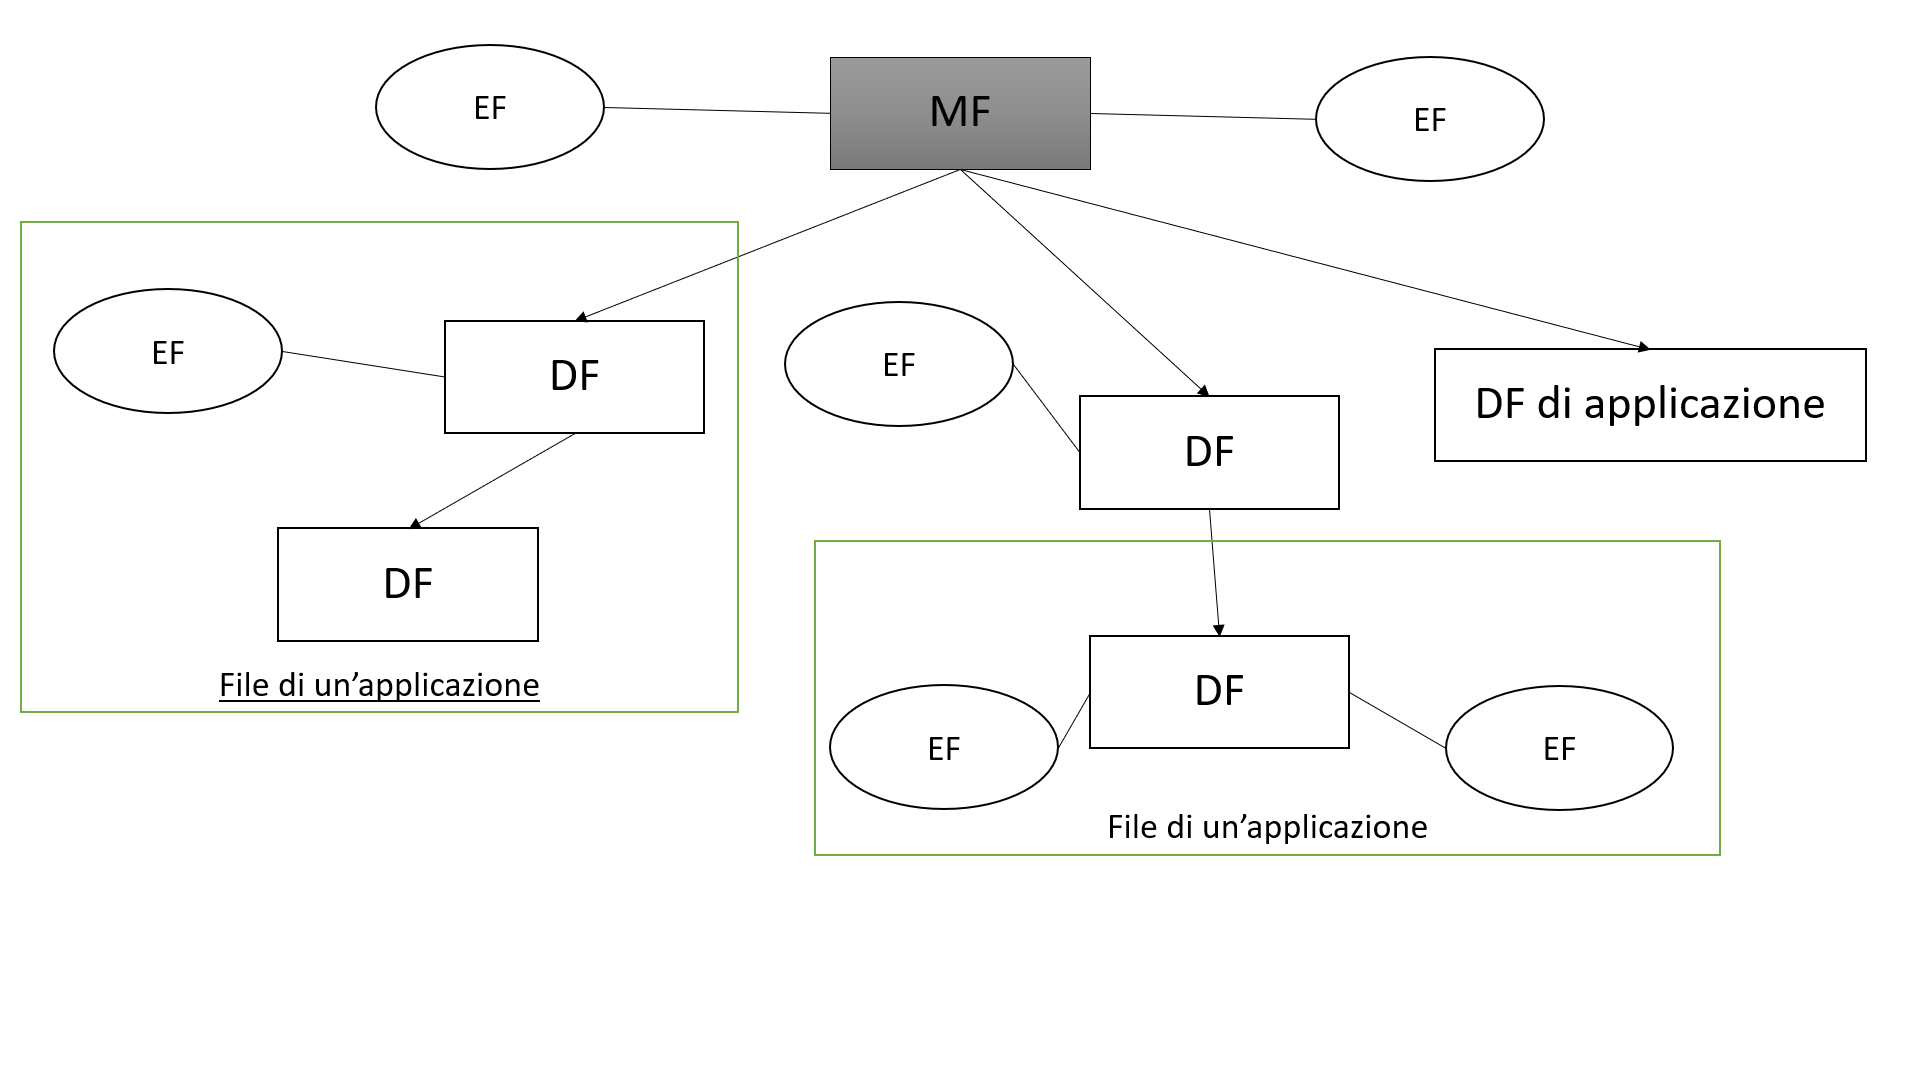
\includegraphics[width=400pt]{pictures/gerarchia_file.png}
  \caption{Esempio di una gerarchia di file in una smartcard.}
  \label{fig:file_system}
\end{figure}

\subsubsection{Sicurezza}
L'accesso ai file è, naturalmente, protetto. Lo standard fa riferimento a uno stato di sicurezza ovvero uno stato che è possibile ottenere al seguito di una procedura di autenticazione nella quale viene richiesta, ad esempio, la conoscenza di una password o di una key.

Vengono considerate quattro tipologie di stato di sicurezza:
\begin{itemize}
    \item \textbf{Stato di sicurezza globale}, è solitamente legato a una procedura di autenticazione risiedente nel MF e quindi serve per proteggere l'itera struttura del file system.
    \item \textbf{Stato di sicurezza specifico per un'applicazione}, può essere modificato al seguito del completamento di una procedura di autenticazione basata su un'applicazione può essere mantenuto, perso o recuperato quando durante la procedura di selezione di un'applicazione. Questo stato è rilevante solo per l'applicazione alla quale fa riferimento.
    \item \textbf{Stato di sicurezza specifico per un file}, il funzionamento è simile allo stato relativo a un'applicazione, tuttavia lo stato si basa su un DF specifico e può essere mantenuto, perso o recuperato quando viene selezionato un file. Uno stato di sicurezza globale può essere visto come un caso particolare.
    \item \textbf{Stato di sicurezza relativo a un comando}, quest'ultimo stato esiste solo quando viene processato un comando usando una comunicazione sicura che richiede un'autenticazione.
\end{itemize}

Una volta stabilito lo stato in cui si trova chi sta comunicando con la carta, è possibile definire gli attributi di sicurezza, questi definiscono le azioni permesse e le condizioni che devono essere verificate per poterle effettuare. Questi attributi differiscono tra DF e EF e si basano su parametri opzionali presenti in un dato file o nel suo "padre". In particolare questi attributi specificano in quale stato bisogna trovarsi per poter accedere a un dato file e le funzioni (ad esempio \textit{sola lettura}) che sono disponibili quando ci troviamo in un dato stato.

Ultimo aspetto da considerare sono i meccanismi di sicurezza per l'autenticazione. Prima di tutto troviamo l'autenticazione tramite password o tramite key, per la prima la card compara dati inviati dall'esterno con dati segreti presenti al suo interno, mentre per la seconda viene richiesto a chi vuole accedere alla card di mostrare le conoscenza di una chiave privata.

Un altro meccanismo di sicurezza è quello sull'autenticazione dei dati che consiste nell'utilizzo di una chiave segreta o privata per controllare i dati ricevuti dall'esterno. In alternativa la card può usare sempre una chiave segreta o privata per calcolare una checksum o firma digitale da inviare al lettore. Infine l'ultimo meccanismo disponibile e quello della crittografia dei dati, secondo il quale la scheda decifra o cifra dati scambiati con l'esterno usando una chiave segreta o privata.

Se richiesto dall'applicazione i risultati di un'autenticazione possono essere salvati su un file di log interno (EF).
\cite{isoiec3}

%-----------SECTION------------
\section{Java Card}
\label{java_card}
La tecnologia JavaCard permette di realizzare applicazioni in linguaggio Java, dette applet, da far girare sui chip delle smart card in sicurezza. Questa teclogogia è ampiamente utilizzata nel settore delle SIM (di cui un esempio è riportato nel paragrafo \ref{applet_sim}) e delle carte bancarie.
\cite{Wiki_java}

Con l'ausilio del manuale ufficiale pubblicato da Oracle \cite{javacard3platform} verrà illustrata sinteticamente la piattaforma \textbf{Java Card 3} ovvero un kit di sviluppo per applet Java Card.
\subsection{Architettura della piattaforma}
L'architettura classica della piattaforma è costruita su una classica macchina virtuale java.

Il kit di sviluppo include anche un simulatore (\textit{Java Card RE}) che simula l'ambiente che si avrebbe su una carta fisica e implementa le specifiche dello stadard ISO:7816-4:2013 che è trattato più approfonditamente nel paragrafo \ref{standard}. Il simulatore supporta anche venti canali logici e le estensioni APDU (\textit{Application Protocol Data Units}) definite nello standard ISO 7816-3.
\subsubsection{Java Card TCK}
Nel kit di sviluppo fornito da Oracle viene anche fornita una suite di test automatica e configurabile chiamata \textit{Java Card Technology Compatibility Kit} atta a verificare la compatibilità tra l'applet che si stà sviluppando e le specifiche della carta sulla quale la si vuole far girare.

\subsection{Sviluppo degli applet}
Lo sviluppo delgi applet può essere effettuato tramite l'ide Eclipse installando l'\textit{Eclipse Java Card Plug-in}.

I passaggi per lo sviluppo di un applet sono i seguenti:
\begin{itemize}
    \item Installare e impostare l'ambiente di sviluppo usando l'IDE Eclipse e il Plug-in
    \item Prendere familiarità con gli esempi.
    \item Sviluppare l'applet.
    \item Fare il debugging dell'applet.
    \item Creare il file CAP che può essere scaricato sul simulatore o su una card compatibile. Il file viene inviato tramite APDU. Il kit offre un convertitore utilizzabile per generare file CAP da inviare alla scheda (vedere il paragrafo \ref{cap}).
\end{itemize}

\subsection{Utilizzo dei file CAP}
\label{cap}
Per essere installato su una smart card un applet deve essere convertito in Converted Applet (CAP). Per generare questo tipo di file il kit mette a disposizione un convertitore.


Un file CAP utilizza il formato JAR (Java Archive) e, oltre a varie informazioni sul pacchetto Java, contiene un manifesto (\textit{META-INF/MANIFEST.MF}) che fonrnisce una serie di informazioni riguardanti il file. Queste informazioni possono essere usate per facilitare la distribuzione del file.

Le informazioni presenti nel file sono presentate con lo standard \textit{nome:valore} e sono riportate nella tabella \ref{parametri_manifesto}.

\begin{table}[h!]
\centering
\begin{tabular}{ |c|l| } 
 \hline
 \textbf{Nome} &  \textbf{Descrizione del valore} \\
 \hline
 Java-Card-Creation-Time &  Indica quando è stato generato il file CAP \\
 \hline
 Java-Card-Converter-Version & Indica la versione del convertitore utilizzata \\ 
 \hline
 Java-Card-Converter-Provider & Indica il fornitore del convertitore \\ 
 \hline
 Java-Card-File-Version & Versione del file CAP \\
  & secondo la convenzione \textit{maggiore.minore} \\ 
 \hline
 Java-Card-Package-Version & Versione del pacchetto file CAP\\
  & secondo la convenzione \textit{maggiore.minore} \\ 
 \hline
 Java-Card-Package-AID & AID (\textit{JADE Agent Identifier}) del pacchetto \\
 \hline
 Java-Card-Package-Name & Il nome del pacchetto \\
 \hline
 Java-Card-Applet-$<$n$>$-AID & AID (\textit{JADE Agent Identifier}) dell'applet \textit{n}\\
 \hline
 Java-Card-Applet-$<$n$>$-Name & Il nome breve della classe \textit{n} \\
  & implementata dal CAP \\
 \hline
 Java-Card-Import-Package-$<$n$>$-AID & AID (\textit{JADE Agent Identifier})\\
  & del pacchetto \textit{n} importato \\
 \hline
 Java-Card-Import-Package-$<$n$>$-Version & Versione del pacchetto \textit{n} importato\\
  & secondo la convenzione \textit{maggiore.minore}\\
 \hline
 Java-Card-Integer-Support-Required & Può assumere valori \textit{TRUE} o \textit{FALSE}.\\
  & Il valore vero indica che il pacchetto\\
   & richiede l'integer support \\
 \hline
 
\end{tabular}
\caption{Tabella dei parametri presenti nel manifesto del file.}
\label{parametri_manifesto}
\end{table}

\subsubsection{Generazione di un file CAP}
Per generare un file CAP è possibile utilizzare il tool \textit{capgen} fornito dal kit.

Per avviare il tool è possibile usare il comando
\begin{center}
    \textit{capgen.bat \textbf{[opzioni] nome\_del\_file}}.
\end{center}

Le opzioni disponibili sono:
\begin{itemize}
    \item \textbf{-help} che stampa un messaggio di aiuto
    \item \textbf{-nobanner} che sopprime i vari messaggi
    \item \textbf{-o \textit{nome\_del\_file}}.
\end{itemize}
 
\subsection{Fare il debugging delle applicazioni}
Per effettuare il debugging delle applicazioni il kit offre due tool che lavorano insieme per alleggerire la procedura, altrimenti troppo impegnativa per la virtual machine del simulatore.

Il primo tool, \textit{cref} può essere lanciato direttamente da Eclipse o da riga di comando e ha la possibilità di simulare la memoria persistente (EEPROM) nonché di salvare e recuperare i dati salvati sulla memoria o su file presenti sull'hard disk. Inoltre il tool può eseguire operazioni di I/O tramite un'interfaccia socket che simula il collegamento tra il lettore di carte e il computer.

Per il debugging l'IDE utilizza il Java Debug Wire Protocol (JDWP) che, come accennato, è troppo pesante per la piccola VM utilizzata dal simulatore fornito dal kit. Per questo per il debugging viene utilizzato un protocollo proprietario più leggero.

Il secondo tool offerto è il \textit{debugproxy}, esso ha il compito di tradurre comandi e risposte tra l'IDE e il simulatore \textit{cref} utilizzando il protocollo appropriato.

Dato che i tool \textit{cref}, \textit{debugproxy} e l'IDE comunicano tramite socket, essi possono girare su host diversi.

Da Eclipse è possibile far partire il debug proxy per impostare breakpoints, leggere o ipostare variabili e fare il debug di una libreria.

\subsection{Distribuire le proprie applicazioni}
Il kit permette di scaricare un Java Card technology package, effettuare il collegamento con la card, eliminare applets e pacchetti dalla smart card e impostare le applet di default per i vari canali logici.

Per installare l'applicazione su una card bisogna prima convertire i file .class in file .cap utilizzando il convertitore fornito dal kit, successivamente il tool \textit{scriptgen}, ovvero l'off-card installer converte il file .cap in uno script .scr che consiste in una serie di comandi APDU che vengono eseguiti dall'APDUtool. Infine l'on-card installer processa il file CAP e invia gli APDU di risposta all'APDUtool con lo stato ed eventuali dati.

Il file .scr contiene comandi e C-APDU che sono terminati da un punto e virgola.
La sintassi di un C-APDU è la seguente:
\begin{center}
    $<$CLA$>$ $<$INS$>$ $<$P1$>$ $<$P2$>$ $<$LC$>$ [$<$byte 0$>$...$<$byte LC-1$>$] $<$LE$>$;
\end{center}
dove
\begin{itemize}
    \item $<$CLA$>$ è il byte della classe definito dallo standard ISO 7816-4.
    \item $<$INS$>$ è il byte di istruzione definito dallo standard ISO 7816-4.
    \item $<$P1$>$, $<$P2$>$ sono i parametri P1 e P2 definiti dallo standard ISO 7816-4.
    \item $<$LC$>$ è il numero dei byte inviati (1 in modalità non estesa, 2 in modalità estesa).
    \item $<$byte 0$>$...$<$byte LC-1$>$ sono i byte per i dati di input.
    \item $<$LE$>$ è la lunghezza che ci si aspetta per l'output (1 in modalità non estesa, 2 in modalità estesa).
\end{itemize}

Il protocollo utilizzato per installare un applet è composto da una sequenza di comandi ben precisa. Per prima cosa viene inviato un comando di selezione utilizzato per invocare l'on-card installer, segue un comando di CAP Begin. Successivamente viene ripetuta una seria di 3 comandi per ogni componente presente nel file CAP (Component \#\# Begin, Component \#\# Data, Component \#\# End). La sequenza viene conclusa dai comandi CAP End e Create Applet. Ogni comando viene inviato alla card e riceve una risposta che varia a seconda del comando.

\section{Smart Cart Web Server}
Uno \textit{Smart Card Web Server} (SCWS) è un server HTTP implementato all'interno di una smart card, di solito integrata in uno smartphone (SIM - vedi paragrafo \ref{applet_sim}). Questa tecnologia permette agli operatori di telefonia mobile di offrire determinati servizi utilizzando il diffusissimo protocollo \textit{HTTP/1.1}.

Il principale obiettivo di questa tecnologia è quello di creare una comunicazione interna al dispositivo tra un WEB browser che gira nello smartphone e un server presente sulla card. Permette, inolte, un'amministrazione remota della smart card da un'entità autorizzata (ad esempio il fornitore del servizio di telefonia e/o della card stessa).

L'interfaccia HTTP offerta dalla card si trova a un livello logico separato dall'interfaccia di comunicazione definita dallo standard ISO 7816 (vedi paragrafo \ref{standard}) e permette ad applicazioni HTTP di comunicare con la card in maniera autonoma.

Questo canale di comunicazione è utilizzato dai fornitori per offrire maggiori servizi ai loro clienti.

L'URL utilizzato per la comunicazione deve corrispondere alla definizione data dal protocollo \textit{HTTP/1.1}, ovvero

\begin{center}
    http\_URL = "http:" "//" host [ ":" port ] [ abs\_path [ "?" query ]]
\end{center}

La $<query>$ opzionale deve essere una sequuenza di uno o più termini della forma $<name>=<value>$ separati da un '\&'. Il server deve poter rispondere per lo meno a url di 1024 caratteri e \textit{abs\_path} di 128 caratteri.

\subsection{I protocolli di trasporto}
Se la card non ha il proprio indirizzo IP e quindi non supporta il protocollo TCP/IP viene utilizzato il protocollo \textit{ Bearer Independent protocol} (BIT). In particolare, nel client viene fatto girare un gateway BIT che effettua una "traduzione" tra i due protocolli (TCP/IP e BIT). Il protocollo BIT è utilizzato per comunicare tra il gateway e la scheda.

L'IP utilizzato per accedere al gateway è 127.0.0.1, meglio come conosciuto come localhost. Il gateway BIP ascolta sulle porte definite dallo SCWS, solitamente si usano le porte 3516 e 4116, la prima è riservata come "porta della smart card", la seconda come "smart card TLS".

Un esempio di url che può essere utilizzato per accedere a una risorsa chiamata "foobar.xhtml" e presente nel percorso "pub/files" è il seguente:
\begin{center}
    http://127.0.0.1:3516/pub/files/foobar.xhtml 
\end{center}

Mentre il seguente url può essere utilizzato per avviare un'applicazione e passarle dei parametri:
\begin{center}
    http://127.0.0.1:4116/cgi/SSO?account=username\&otherparam=123 
\end{center}

Se la smart card ha il proprio indirizzo IP e quindi supporta il protocollo TCP/IP allora il dispositivo mobile ha la possibilità di comunicare direttamente con la card senza dover passare per un gatway BIT.

La connessione è definita dallo standard ETSI TS 102 483]. L'indirizzo IP per comunicare con la card può essere dinamico, tuttavia ci si riferisce chiamandolo “localuicc”. Le porte per la comunicazione sono la 80 per l'HTTP e la 443 per L'HTTP con TLS (presentato le paragrafo \ref{tls}).

Un paio di URL di esempio sono riportati in seguito:
\begin{center}
    http://localuicc/pub/files/foobar.xhtml
    https://localuicc/cgi/display?df=7F01\&ef=3F01\&record=01\&offset=50\&length=10 
\end{center}

\subsection{Sicurezza della comunicazione}
\label{tls}
Per la sicurezza della trasmissione dei dati con la card viene utilizzato il protocollo \textit{Transport Layer Security}  (TLS). Questo protocollo fornisce un meccanismo sicuro ed affidabile per il trasporto dei dati tra due entità, con un controllo dell'integrità e della confidenzialità delle informazioni scambiate. Fornisce anche dei meccanismi di autenticazione per una o entrambe le parti.

Il TLS è pesato per un paradigma Client-Server dove il client è chi inizia la comunicazione (o invia una richiesta) e il server fornisce una risposta. Solitamente il client può autenticare il server utilizzando un certificato a chiave pubblica. Un'auntenticazione mutua può essere effettuata utilizzando dei certificati a chiave pubblica pre-condivisi (\textit{Pre Shared Keys-TLS} o PSK-TLS)
\cite{scwebserver}
\chapter{Token crittografici}
\label{chapter3}



\chapter*{Conclusione}
\label{epilogue}
\addcontentsline{toc}{chapter}{Conclusione}
Il mondo delle Smart Card e dei Token crittografici è enorme e in continua evoluzione, data l'importanza e la delicatezza dei problemi che si vogliono risolvere con queste tecnologie.

In questa tesi è stato fatto una breve panoramica di concetti molto importanti, ognuno dei quali richiederebbe un libro a parte per essere trattato in maniera sufficientemente approfondita.

Si spera che chi è interessato al settore della sicurezza informatica abbia si sia incuriosito degli argomenti accennati e, aiutandosi con la bibliografia, riesca a soddisfare la propria curiosità.

\medskip

%Sets the bibliography style to UNSRT and imports the 
%bibliography file "samples.bib".
\bibliographystyle{unsrt}
\bibliography{references}

\end{document}
